\documentclass[border=10pt]{standalone}

\usepackage{tikz}
\usepackage{tikzsymbols}
\usetikzlibrary{calc,patterns,shapes.geometric}

\def\centerarc[#1](#2)(#3:#4:#5){\draw[#1] ($(#2)+({#5*cos(#3)},{#5*sin(#3)})$) arc (#3:#4:#5);}

\begin{document}
	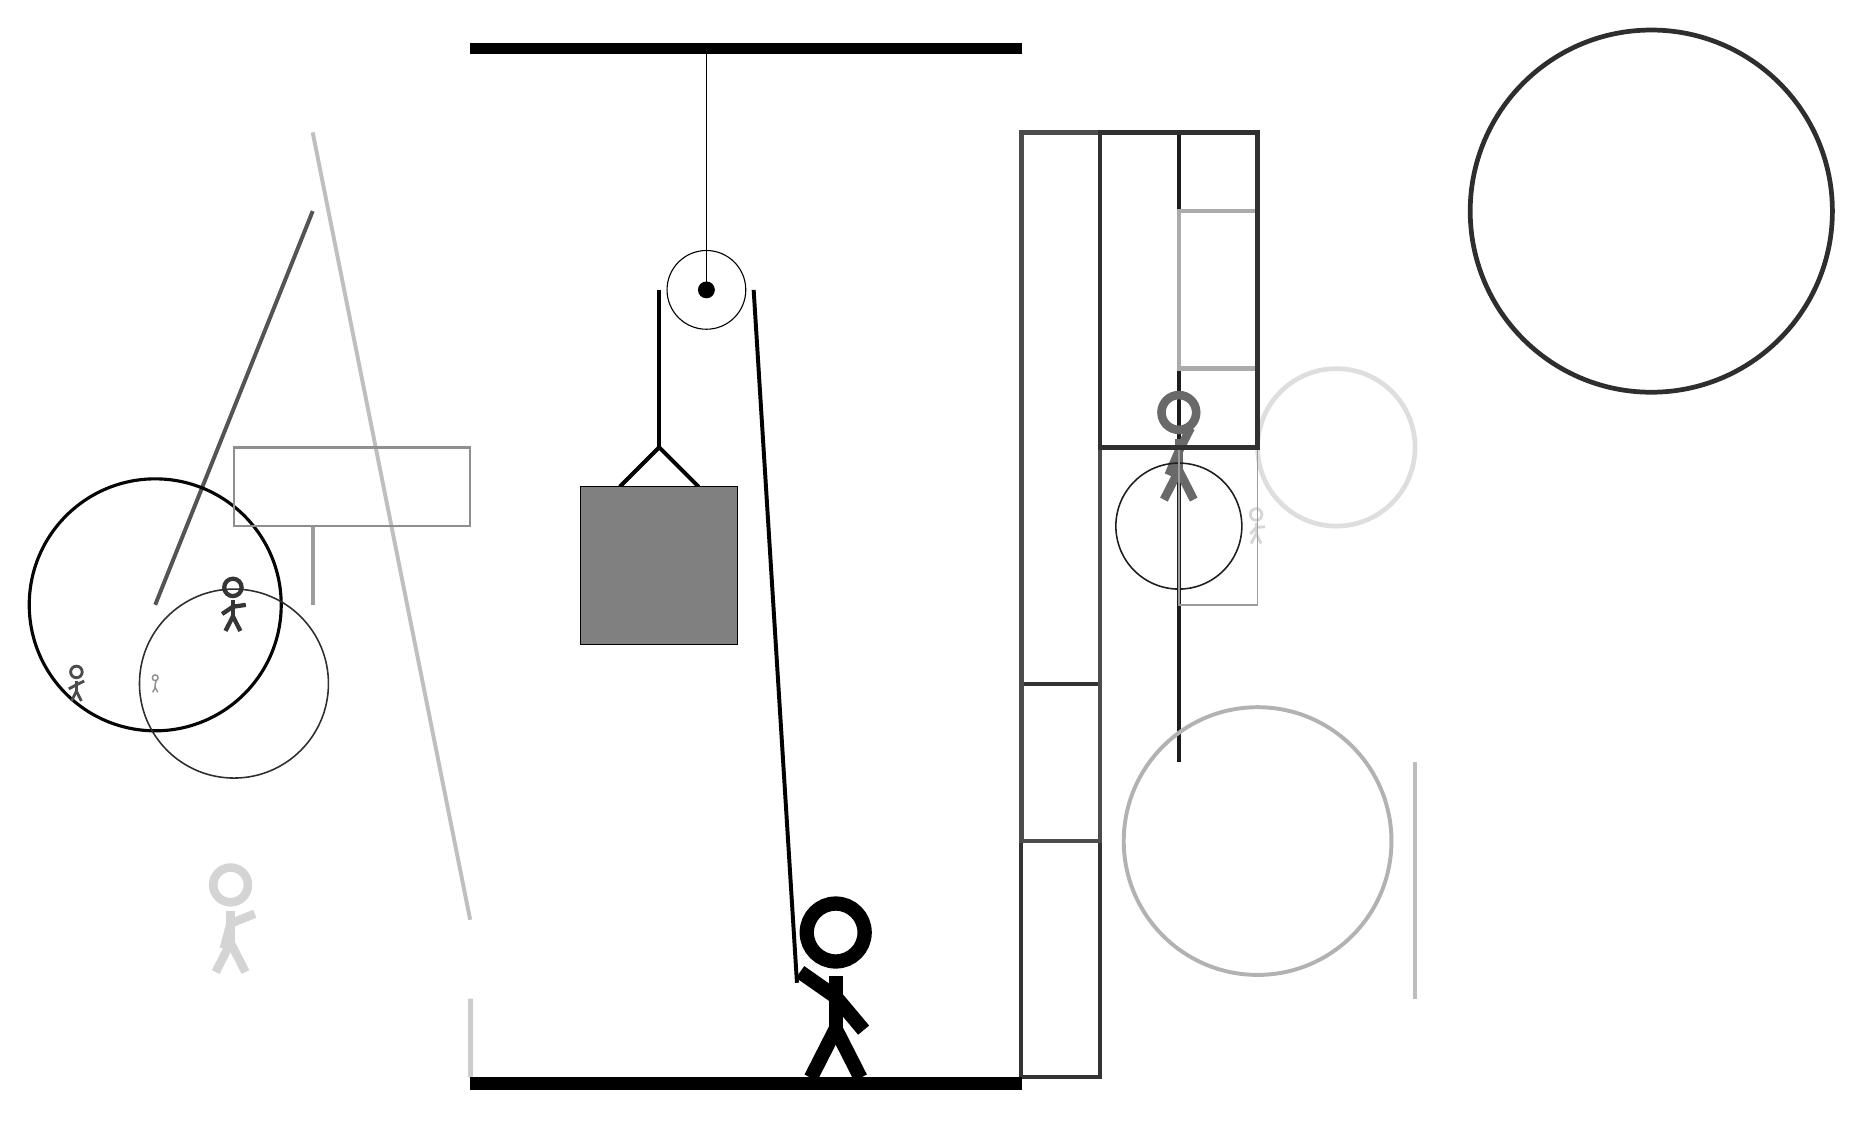
\begin{tikzpicture}
		%%%%% START %%%%%
		
		\draw[fill=black] (-2, 10) rectangle (5, 10.125);
		
		\draw (1, 7) circle (0.5);
		\draw[fill=black] (1, 7) circle (0.1);
		\draw (1, 10) -- (1, 7);
		
		\draw[line width=0.5mm, color=black!67](-4, 8) -- (-6, 3);
		
		\draw[line width=0.5mm, color=black!89](7, 1) -- (7, 9);
		\draw[line width=0.5mm, color=black!25](-4, 9) -- (-2, -1);
		\draw[line width=0.6mm, color=black!20] (-2, -2) rectangle (-2, -3);
		\node[line width=0.3mm, color=black!44] at (-6, 2) {\Strichmaxerl[1][85][75]};
		
		\node[line width=0.2mm, color=black!79] at (-5, 3) {\Strichmaxerl[3][34][8]};
		\draw [line width=0.4mm, color=black!98](-6, 3) circle (1.6);
		\draw [line width=0.6mm, color=black!82](13, 8) circle (2.3);
		\node[line width=0.4mm, color=black!16] at (8, 4) {\Strichmaxerl[2][49][3]};
		\node[line width=0.7mm, color=black!17] at (-5, -1) {\Strichmaxerl[6][75][22]};
		\draw [line width=0.6mm, color=black!13](9, 5) circle (1.0);
		\draw [line width=0.5mm, color=black!30](8, 0) circle (1.7);
		\node[line width=0.4mm, color=black!59] at (7, 5) {\Strichmaxerl[6][67][63]};
		\draw[line width=0.5mm, color=black!80] (5, -3) rectangle (6, 2);
		\draw[line width=0.6mm, color=black!70] (5, 9) rectangle (6, 0);
		\draw[line width=0.5mm, color=black!39](-4, 4) -- (-4, 3);
		
		\draw[line width=0.3mm, color=black!44] (-2, 4) rectangle (-5, 5);
		\draw[line width=0.6mm, color=black!33] (7, 6) rectangle (8, 8);
		\draw [line width=0.2mm, color=black!88](7, 4) circle (0.8);
		
		\draw[line width=0.2mm, color=black!39] (7, 3) rectangle (8, 5);
		\node[line width=0.7mm, color=black!70] at (-7, 2) {\Strichmaxerl[2][28][26]};
		
		\draw [line width=0.2mm, color=black!82](-5, 2) circle (1.2);
		\draw[line width=0.6mm, color=black!81] (6, 9) rectangle (8, 5);
		\draw[line width=0.5mm, color=black!26](10, 1) -- (10, -2);
		
		\draw[line width=0.5mm] (-0.1, 4.5) -- (0.4, 5.0) -- (0.9, 4.5);
		\draw[fill=black!50] (-0.6, 4.5) rectangle (1.4, 2.5);
		
		\draw[line width=0.5mm] (0.4, 7) -- (0.4, 5.0);
		\centerarc[line width=0.5mm](1, 7)(0:180:0.6);
		\draw[line width=0.5mm](1.6, 7) -- (2.15, -1.8);
		
		\node at (2.6, -1.9) {\Strichmaxerl[10][-35][-50]};
		
		\draw[fill=black] (-2, -3) rectangle (5, -3.15);
		
		%%%%% END %%%%%
	\end{tikzpicture}
\end{document}